\chapter{Choosing a Prediction Model}
\thispagestyle{nohead}
\label{Prediction}

This chapter will evaluate the effectiveness of a number of machine learning algorithms at predicting the most appropriate SMT solver to use on any (unseen) \textsf{Why3} PO.
Our goal in this thesis is to construct a ``meta-solver'' or \textit{portfolio} solver which chooses from a range of tools in order to prove more goals than a single solver is capable of.
We motivate the need for a portfolio solver with an analysis of our dataset 
in Sec. \ref{sec:portfolio-benefit}. 
More details about the type of prediction task chosen for the evaluation of ML algorithms is given in Sec. \ref{sec:reg-class}.
A more detailed introduction to the six prediction algorithms (some of which were introduced previously in Sec. \ref{sec:lrml} and Table \ref{table:algorithms}) is given in Sec. \ref{pred:choosing} before the results of their comparison is discussed. 
We make this comparison with reference to a number of theoretical strategies introduced in Sec. \ref{sec:strategies}.
We end this chapter with a more detailed look at the model chosen for use in the actual implementation of \where.

Throughout this chapter, we use the terms ``algorithms'' and ``models'' to refer to different, but related, concepts. An ``algorithm'' refers to the general approach to prediction, as formalised to be applicable to a number of prediction scenarios.
``Models'' are trained instances of these algorithms which use specific parameters and data to make predictions for a single use case.

\section{The benefit of portfolio-solving in \why}
\label{sec:portfolio-benefit}

\newcolumntype{Z}{>{\raggedleft\arraybackslash}X} 
\begin{table}
	\caption[Results of running eight solvers on the example \textsf{Why3} programs]{Results of running eight solvers on the example \textsf{Why3} programs.  Also included is a theoretical solver  \textsf{Choose Single}, which always returns the best answer in the fastest time.}
	\begin{tabularx}{1.1\textwidth}{@{}l|ZZZ|ZZZ|ZZZ@{}}
		\toprule
		{} & \multicolumn{3}{c|}{\textbf{File}} & \multicolumn{3}{c|}{\textbf{Theory}} & \multicolumn{3}{c}{\textbf{Goal}} \\
		{} & \# proved & \% proved & Avg time & \# proved & \% proved & Avg time & \# proved & \% proved & Avg time \\
		\midrule
		\textsf{Choose Single} & \textbf{48} & \textbf{37.5\%} & \textbf{1.90} & \textbf{190} & \textbf{63.8\%} & \textbf{1.03} & \textbf{837} & \textbf{79.9\%} & \textbf{0.42} \\
		\textbf{Alt-Ergo-0.95.2} & 25 & 19.5\% & 1.45 & 118 & 39.6\%& 0.77 & 568 & 54.2\% & 0.54 \\ 
		\textbf{Alt-Ergo-1.01} & 34 & 26.6\% & 1.70 & 142 & 47.7\% & 0.79 & 632 & 60.3\% & 0.48 \\ 
		\textbf{CVC3} & 19 & 14.8\% & 1.06 & 128 & 43.0\% & 0.65 & 597 & 57.0\% & 0.49 \\ 
		\textbf{CVC4} & 19  & 14.8\% & 1.09 & 117 & 39.3\% & 0.51 & 612 & 58.4\% & 0.37 \\ 
		\textbf{veriT} & 5 & 4.0\% & 0.12 & 79 & 26.5\% & 0.20 & 333 & 31.8\% & 0.26 \\ 
		\textbf{Yices} & 14 & 10.9\% & 0.53 & 102 & 34.2\% & 0.22 & 368 & 35.1\% & 0.22 \\ 
		\textbf{Z3-4.3.2} & 25 & 19.5\% & 0.56 & 128 & 43.0\% & 0.36 & 488 & 46.6\% & 0.38 \\ 
		\textbf{Z3-4.4.1} & 26 & 20.3\% & 0.58 & 130 & 43.6\% & 0.40 & 581 & 55.4\% & 0.35 \\ 
		\bottomrule
	\end{tabularx}
	\label{table:avgtimes}
\end{table} 
%
%\begin{table}
%	\centering
%	\caption[Number of trivial and hard \textsf{Why3}verification tasks]{Number of trivial and hard \textsf{Why3}verification tasks}
%	\begin{tabularx}{0.8\textwidth}{@{}l|ZZZ@{}}
%		{} & \multicolumn{1}{r}{\textbf{File}} & \multicolumn{1}{r}{\textbf{Theory}} & \multicolumn{1}{r}{\textbf{Goal}} \\	
%		\midrule
%		\textbf{Trivial} (all solvers can prove) & 3 & 55 & 206 \\
%		\textbf{Hard} (no solver can prove) & 85 & 118 & 211 \\
%	\end{tabularx}
%	\label{table:trivial-hard}
%\end{table} 

\begin{table}
	\centering
	\caption[Breakdown of results in terms of triviality and hardness]{Breakdown of results in terms of triviality and hardness}
	\begin{tabularx}{0.9\textwidth}{@{}l|ZZZ@{}}
		{} & \multicolumn{1}{r}{\textbf{File}} & \multicolumn{1}{r}{\textbf{Theory}} & \multicolumn{1}{r}{\textbf{Goal}} \\	
		\midrule
		
		\textbf{Trivial} (all solvers can prove) & 3 & 55 & 206 \\
		\textbf{Hard} (no solver can prove) & 85 & 118 & 211 \\
		\midrule
		\multicolumn{4}{c}{\textsc{Uniquely-provable by a single solver}} \\
		\midrule
		\textbf{Alt-Ergo-0.95.2} & 0 & 0 & 1 \\ 
		\textbf{Alt-Ergo-1.01} & 6 & 12 & 25 \\ 
		\textbf{CVC3} & 2 & 3 & 17 \\ 
		\textbf{CVC4} & 1 & 6 & 33 \\ 
		\textbf{veriT} & 0 & 0 & 0 \\ 
		\textbf{Yices} & 0 & 0 & 2 \\ 
		\textbf{Z3-4.3.2} & 0 & 0 & 0 \\ 
		\textbf{Z3-4.4.1} & 0 & 0 & 2 \\ 
		\midrule
		\textbf{Others}: provable by at least two, & 32 & 104 & 551 \\
		but not all, solvers & & & \\
		\midrule
		\textsc{total} & 129 & 298 & 1048 \\
		\bottomrule
	\end{tabularx}
	\label{table:unique}
\end{table} 


Now that the SMT solvers to be supported by \textsf{Where4} have been identified and an appropriate dataset for training and testing purposes has been chosen, we can make a preliminary and exploratory analysis of the behaviour of the SMT tools on the particular data. 
We aim to make a case for portfolio-solving as an effective method for discharging POs in the \textsf{Why3} system.

We refer the reader to Table \ref{table:avgtimes} which shows the results of running eight solvers on the example \textsf{Why3} programs with a timeout value of ten seconds. 
The entire dataset is used in this case. 
WhyML files are modularised as one or more complete \textit{theories} which can be used locally by other theories in the same file. 
The \textsf{Why3} IVL identifies the \textit{goals} which need to be proven in order for the theory (and in turn the entire file) to be verified as correct.
WhyML theories containing assertions and lemmas can produce many goals while others which merely define types and helper functions can produce none. 
Our dataset of 128 WhyML files consists of 289 theories, which in turn generate 1048 goals. 
Aside from the number of each modular construct proved by the solver (\textit{left sub-column}), the percentage this number represents of the total is given (\textit{centre sub-column}) and the average time taken (in seconds) to prove each construct (as measured using the process described in Sec. \ref{sub:confidence}) is given in the \textit{right sub-column}. 

We show the results of proving a WhyML file using its modular constructs. 
This method of verification is particularly useful when \textsf{Why3} is run in batch mode from the command line.
%It is more natural to select separate solvers on a per-goal basis through the \textsf{Why3}IDE which breaks each WhyML program into theories and goals automatically. 
When using the \textsf{Why3} IDE, it is more natural to prove programs by applying solvers to individual goals.
This is because the environment separates WhyML programs into theories and goals automatically.

Table \ref{table:avgtimes} also shows the results for a theoretical solver \textsf{Choose Single}. 
\textsf{Choose Single} is the best solver, from the eight SMT solvers measured, chosen on a per-goal basis. 
For example, if a file contains one theory which consists of three goals, and the best-performing solver is CVC4 for the first goal, Yices for the second, and CVC3 for the third, the result for \textsf{Choose Single} on that file is the sum of the results for CVC4 on the first goal, Yices on the second, etc.
We define what is means for a solver to be the \textit{best} in the next subsection.

The theoretical solver \textsf{Choose Single} shows the benefit of being able to use the most appropriate solver for each PO: 205 more goals are provable -- an increase of 19.6\% -- over the best single solver (Alt-Ergo version 1.01) which can prove a total of 632. 
In total, 837 goals are provable by using a combination of the eight solvers -- a figure that represents 79.9\% of the 1048 goals. 
On average, \textsf{Choose Single} proves goals in a shorter amount of time than either version of Alt-Ergo or CVC3. 
The average time subcolumn provides an insight into how solvers which can prove relatively few goals, theories, or entire files -- such as veriT or Yices -- can be useful in a portfolio-solving context: such solvers often prove what they can in a very short amount of time (veriT takes an average time of just 0.12 seconds, for example, to prove each of five entire files) and can be the best choice of solver for those files, theories and goals. 

The advantages of using multiple solvers are further illustrated by the results presented in Table \ref{table:unique}. \textit{Trivial} files, theories and goals (the first row of Table \ref{table:unique}) are defined as those which can be proved by all eight solvers measured. 
Three files, 55 theories and 206 goals fall under the trivial category.
Again, this table provides an interesting insight into the behaviour of all solvers: three of the five files proved by veriT are trivially provable by all solvers (which may explain the short amount of time taken, on average, to prove the five files). 
The second row of this table shows the number of \textit{hard} files, theories and goals. 
These are the tasks which no solver is able to prove entirely.
As we have previously discussed in Sec. \ref{sub:prover-output}, these goals usually require the use of an ITP or splitting transformation to be discharged.
Two hundred and eleven goals fall under this category.

The breakdown of the number of files, theories and goals which \textit{only one} solver is able to prove is given in Table \ref{table:unique}.
The good performance of Alt-Ergo version 1.01 is obvious: six complete files can only be proved in their entirety by the solver. 
A higher number of goals require the use of CVC4 in order to be proved, however.
Thirty-three goals (compared to twenty-five for the newer version of Alt-Ergo) can \textit{only} be proved by this solver.
The relatively low numbers for files, theories and goals provable by a single solver suggests that most goals can be proved by more than one tool, if they can be proved at all.
Indeed, the second-to-bottom row of Table \ref{table:unique} shows that the majority of goals fall in this category. 

\subsection{The relative utility of solver responses}
\label{sub:rel-util}

To make assertions about the relative performance of different solvers on the same goal, a definition of the relative \textit{utility} of solver responses is required.
Should a solver which returns an answer of \textit{Valid} in five seconds be seen as ``worse'' than one that returns \textit{Unknown} in half a second? 
Likewise, should the solver returning \textit{Failure} after one second be penalised more severely than one returning \textit{Timeout} after the maximum time limit?

We define an ordering for response utility as 
\[
\lbrace Valid, Invalid\rbrace > Unknown > \lbrace Timeout, Failure\rbrace
\]  
the reasoning being that a \textit{Failure} response usually signals a fatal error in the logic encoding for that solver/goal pair, and the learning algorithm should be discouraged from choosing a failing solver for the particular goal characteristics in question. 
As discussed in Sec. \ref{sub:timeout-limit} of the previous chapter, \textit{Unknown} answers are returned quickly in general, and should not be penalised as much as \textit{Timeout} responses. 
Solvers which reach the timeout limit are unlikely to return a \textit{Valid} or \textit{Invalid} response if given more time (illustrated clearly by Fig. \ref{fig:line_graph}).
Solvers returning the same answer are ranked according to runtime -- with faster solvers being preferred.

This method for defining relative performance has similarities to the scoring structure for ATPs competing in SV-COMP \cite{Beyer2016, SVCOMP}, with some important differences. 
In SV-COMP, \textit{Unknown} responses are given a neutral score of 0, the correct reporting of a property which does not hold (``true negative") is rewarded with smaller score ($+1$) than the correct reporting of a property which is found to hold (``true positive" which scores $+2$).
Likewise, the incorrect reporting of a property which does not hold (``false negative" or ``false alarm") is punished less severely (with a score of $-4$) than the incorrect reporting of a property which does hold (``false positives" score $-8$).  
Although the notion of ``false positive'' and ``false negative'' responses is not applicable in the SMT domain (where tools are assumed to be sound), we follow the SV-COMP scoring scheme by awarding a ``true positive'' (or \textit{Valid} response) a higher score than a ``true negative'' (or \textit{Invalid} response). 
\textit{Unknown, Timeout} and \textit{Failure} responses are not treated separately by the SV-COMP scoring scheme -- they all fall under the \textit{Unknown} response category.
We penalise poorly-performing solvers through the use of a \textit{cost} function.
%A further refinement to our scoring model was necessary in order for the prediction models to operate effectively. 
The definition of the cost function we applied to solver results is given in Sec. \ref{sub:scoring} of this chapter. 

\section{Classification and regression}
\label{sec:reg-class}

Machine learning prediction tasks can be separated into two categories: those involving the \textit{classification} of a variable into discrete categories or classes, and those predicting a continuous-valued variable directly -- \textit{regression} tasks.
This section will discuss some of the options considered when designing \where's prediction task.

\subsection{Predicting the single best solver} This option involves a multi-class classification task: the classes involved are the eight SMT solvers.
Each PO is classified as belonging in one class. 
We reject this approach because some benefits associated with portfolio-solving are lost, since if the PO is misclassified, the performance of the portfolio solver suffers severely.
For example, the single solver can return an answer of \textit{Failure} with no other solver suggestion being made.
In the best case, the predictions would be equivalent to the \textsf{Choose Single} theoretical solver.

%this method was found to be only marginally better than choosing one of the eight solvers at random. 
\subsection{Predicting the best \textit{ranking} of solvers} Again, this option is a multi-class classification task. 
Instead of predicting a single solver, however, the task involves predicting the entire ranking of eight solvers. 
The benefit of obtaining a ranking is the flexibility it affords in calling SMT solvers sequentially or in parallel.
If the first solver fails or returns an answer other than \textit{Valid} or \textit{Invalid}, the next best predicted solver is called, and so on.

With eight SMT solvers there are eight factorial (or 40,320) rankings which is far too many to be reasonable for a classification task. 
We rejected this approach because in our dataset of 1048 POs many of these rankings could not possibly be represented.
In fact, only 766 of the 40,320 rankings occur in our dataset.  
%Many of these rankings were observed very rarely or did not appear at all in the training data. 
Such an unbalanced representation of classes cannot lead to accurate classification.
\subsection{Predicting solver runtime and response separately}
This approach involves two separate tasks, each predicting a characteristic of the solver's performance. 
One model would attempt to predict the response class (i.e. \textit{Valid, Invalid}, etc.) while another would attempt to predict the solver runtime.
The former task is a multi-class classification task with five classes, while the latter is a multi-output regression task.
This method has the advantage of affording the user flexibility in how to choose the ultimate ranking: for example, if fast responses are preferred over \textit{Valid} answers.
This flexibility comes at the price of complexity, however: two accurate predictors, a classifier and regressor, are required instead of one.
\subsection{Combining the prediction of solver response and runtime}
This option uses a cost function to combine the two solver response variables as a single real-valued number which is used for ranking the solvers.
This is a multi-output regression task: a cost prediction is made for each solver individually.
The individual predicted values are sorted in increasing order to produce a ranking of decreasing ``solver utility''.

This approach shares most of the advantages of predicting solver response and runtime separately: each solver's actual behaviour is predicted directly rather than relying on the relative behaviour of all eight \textit{together} constituting a single class. 
It is relatively simple to change the cost function, although it can not be done ``on-the-fly'' in the same manner as the previous approach allows.
A change to the cost function requires re-training the model.
The major benefit is having one single model to predict both the solver response and the runtime. 
This is the prediction approach chosen for \textsf{Where4} in this thesis.  

\subsection{The Cost Function}
\label{sub:scoring}

The use of a cost function is inspired by the first version of the SATZilla portfolio solver \cite{Satzilla}. 
The cited paper describes the prediction of a \textit{performance score}.
This differs from most portfolio approaches which aim to predict a solver's runtime directly. 

The cost function should reflect the ordering of solver utility defined in Sec. \ref{sub:rel-util}: penalising poorly-performing solvers while ensuring \textit{Valid} and \textit{Invalid} responses incur the lowest cost.
The following simple function allocates a cost to each solver $S$'s response $\langle answer, time\rangle$ to each goal $G$:
\begin{equation}
\label{eq:chosen-cost}
\small
cost(S,G) = 
\begin{cases}
time_{S,G}, \text{ if answer}_{S,G} \in \lbrace Valid, Invalid \rbrace \\
time_{S,G} + \text{timeout}, \text{ if answer}_{S,G} = Unknown \\
time_{S,G} + (\text{timeout} \times 2), \text{ if answer}_{S,G} \in \lbrace Timeout, Failure \rbrace
%dist((time_{S,G},\text{timeout}), (0,0)), \text{if answer}_{S,G} \in \lbrace Timeout, Failure \rbrace
\end{cases}
\end{equation}



Thus, to penalise the solvers that return an \textit{Unknown} result, the timeout limit is added to the time taken, while solvers returning \textit{Timeout} or \textit{Failure} are further penalised by 
adding double the timeout limit to the time taken.
A response of \textit{Failure} refers to an error with the back-end solver and usually means a required logical theory is not supported. 
This function ensures the best-performing solvers always have the lowest costs. A ranking of solvers for each goal in order of decreasing relevance is obtained by sorting the solvers by cost in ascending order.

Other cost functions were trialled before this formulation was decided upon.
Previous methods allocated a cost penalty (based on the answer) and calculated the solver cost as the Euclidean distance from the origin to point defined as this penalty and the solver's time. 
Eg: $cost(S,G) = dist((time_{S,G}, penalty_{ans}),(0,0))$.
Where the penalties associated with each response are:
\begin{equation}
\label{eq:first-cost}
penalty_{ans} = \begin{cases}
0 \text{ if ans} = Valid \\
5 \text{ if ans} = Invalid \\
10 \text{ if ans} = Unknown \\
15 \text{ if ans} = Timeout \\
20 \text{ if ans} = Failure
\end{cases}
\end{equation}
The problem with this formulation is that the penalty values are arbitrarily determined and bear no relation with the timeout value. 
It is therefore not guaranteed that our defined \textit{relative utility} of solvers is respected by using the penalties of Eq. \ref{eq:first-cost}. 
%For example Solver $A$ returning an answer of \textit{Timeout} after 10 seconds would have a cost of $dist((15,10),(0,0)) = 18.03$ whereas Solver $B$ returning a cost of \textit{Failure} after 0.1 seconds (which should have a higher cost than Solver $A$) would have a cost of $dist(())$.  
This issue led us to re-formulate the cost function to incorporate the timeout value as follows:
\begin{equation}
\label{eq:second-cost}
\small
cost(S,G) = 
\begin{cases}
time_{S,G}, \text{ if answer}_{S,G} \in \lbrace Valid, Invalid \rbrace \\
time_{S,G} + \text{timeout}, \text{ if answer}_{S,G} = Unknown \\
dist((time_{S,G},\text{timeout}), (0,0)), \text{if answer}_{S,G} \in \lbrace Timeout, Failure \rbrace
\end{cases}
\end{equation}
which only makes use of the Euclidean distance for \textit{Timeout} and \textit{Failure} responses.
As pointed out by a reviewer of an early version of this work \cite{FIDE2016}, in certain circumstances a \textit{Timeout} response may have a lower cost than an \textit{Unknown} response.
This is the case when the \textit{Unknown} response is returned in a time >= 0.42 times that of the time taken to return a response of \textit{Timeout}. 
This property of the triangle inequality was account for in the final formulation of the cost function (Eq. \ref{eq:chosen-cost}). \\
\\
\textbf{Example: using the cost function to obtain a ranking for \textit{first\_last}}: \\
To illustrate the effect of applying our cost function, we return to the \textit{first\_last} goal introduced in the previous chapter.
Table \ref{table:cost} lists the results of executing the eight solvers on the goal, as measured using the method described in Sec. \ref{sec:dependant}, with a time limit of ten seconds. 
The derived cost value for each solver is used as its dependent variable in the prediction models compared in Sec. \ref{pred:choosing} and \textsf{Where4}'s actual implementation.


\begin{table}
	\caption[Result of eight solver executions on \textit{first\_last} ]{Result of eight solver executions on \textit{first\_last}}
	\begin{tabularx}{\textwidth}{@{}YZZYZY@{}}
		\toprule
		\textsc{Solver} & \textsc{Version} &  \textsc{Runtime (Secs)} & \textsc{Response} & \textsc{Cost} & \textsc{Rank Position} \\
		\midrule
		Alt-Ergo & 	0.95.1 & 	0.134 & 	Unknown & 	10.134 & 2\\
		Alt-Ergo & 	1.10 & 		0.170 & 	Unknown & 	10.171 & 3\\
		CVC3 & 		2.4.1 & 	0.356 & 	Valid & 	0.356 & 1\\
		CVC4 & 		1.4 &		0.173 & 	Unknown  & 	10.173 & 4\\
		veriT & 	201506 & 	10.109 & 	Timeout & 	30.109 & 5\\
		Yices & 	1.0.38 & 	10.161 & 	Timeout & 	30.161 & 8\\
		Z3 & 		4.3.2 & 	10.115 & 	Timeout & 	30.115 & 6\\
		Z3 & 		4.4.1 & 	10.131 & 	Timeout & 	30.131 & 7\\
		%	\midrule
		%	\multicolumn{3}{l}{\textsc{Derived Ranking}:} & & & \\
		%	\multicolumn{4}{l}{CVC3 > Alt-Ergo-0.95.1 > Alt-Ergo-1.01 >} & & \\
		%	& & \multicolumn{4}{r}{CVC4 > veriT > Z3-4.3.2 > Z3-4.4.1 > Yices}  \\
		\bottomrule
		
	\end{tabularx}
	\label{table:cost}
\end{table}
 
\section{Choosing the most effective algorithm for rank prediction}
\label{pred:choosing}


Fig. \ref{fig:Chapter4} illustrates a high-level view of the process used to compare and evaluate the various ranking strategies in this section. 
The solver timings and results are combined as a single variable using the cost function defined in Sec. \ref{sub:scoring}.
The value returned by this function is the response variable for a number of ML algorithms; with the statically-extracted features acting as the predictor variables.

A four-fold cross validation of this data is used to evaluate the models. 
In this method, the data is split into quarters.
Four models are effectively trained on different datasets by holding a different quarter back for model evaluation each time.
The final evaluation is based on the model's average performance over the four instances.
The general \textit{K-fold} cross validation method allows the use of the entire dataset for model evaluation and training (rather than holding a portion of the data back solely for model evaluation use -- a technique known as ``hold-out'' validation). 
The number of folds used (four) was chosen to reflect the percentage of the total dataset (75\%) used for training. 
The folds were stratified (i.e. ensuring a representative frequency of values was contained in each split) according to the best performing solver for each instance.
This technique was used to overcome the difficulties of stratification for regression tasks where values may appear infrequently.  

\begin{figure}
	\centering
	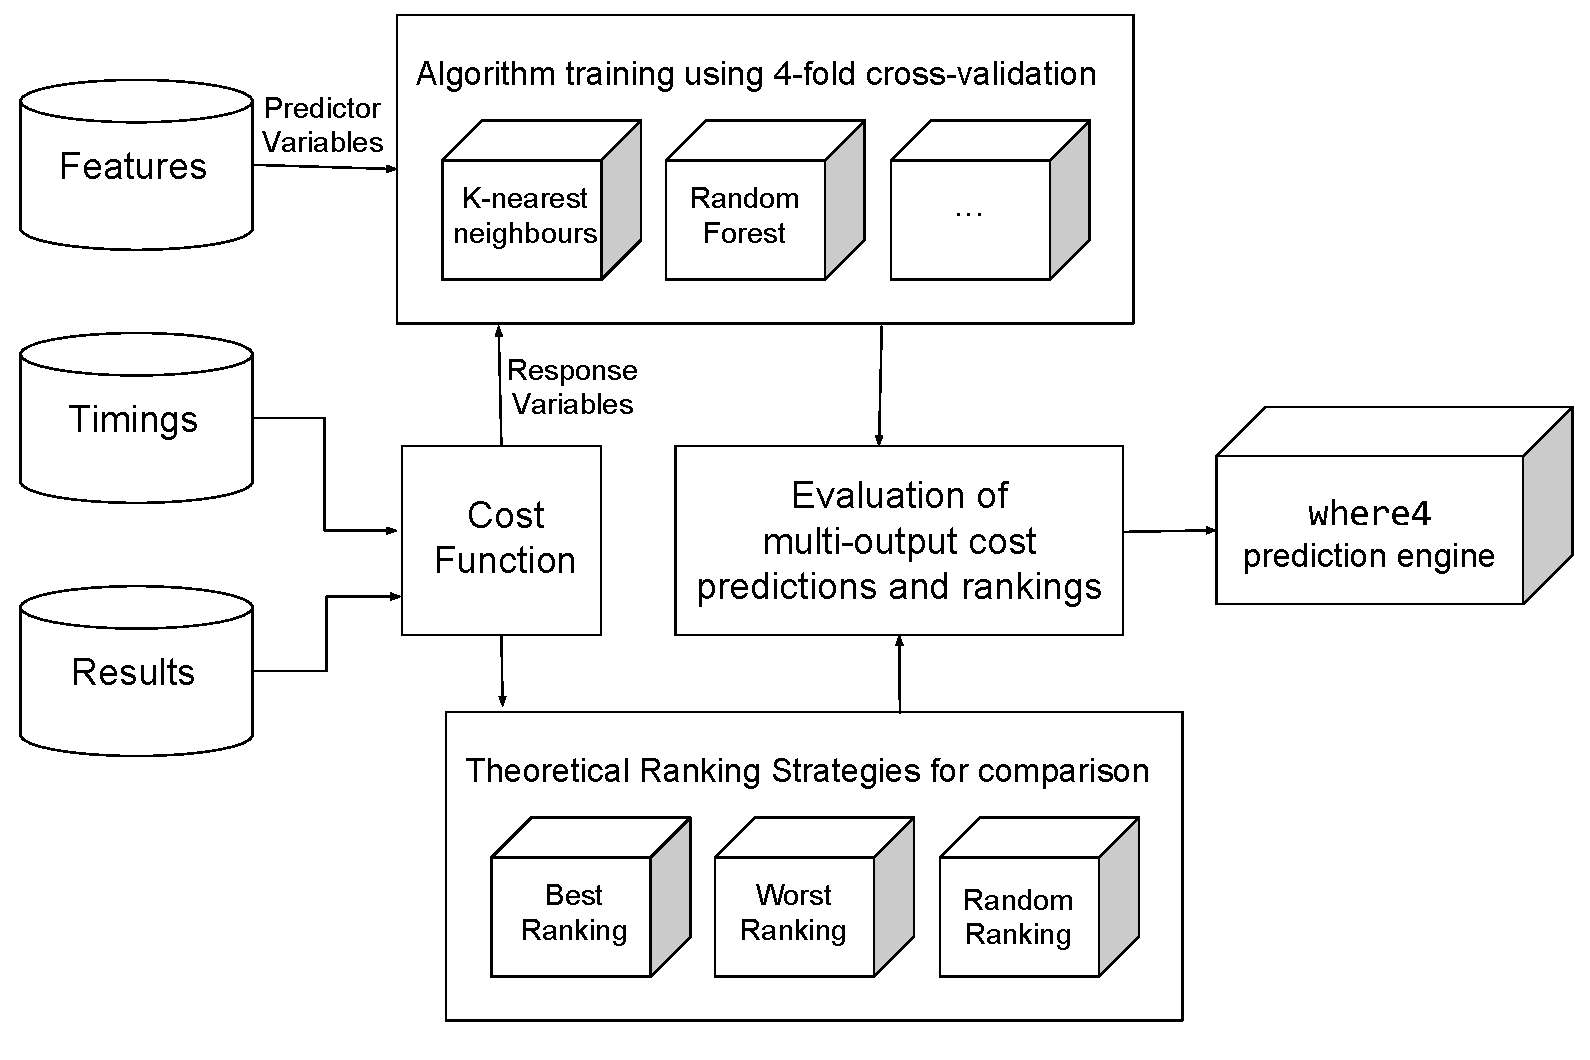
\includegraphics[width=1.0\linewidth]{Figures/Chapter4}
	\caption{Overview of the process used to derive the \textsf{Where4} prediction model}
	\label{fig:Chapter4}
\end{figure}

\subsection{The ML algorithms we used for model training}

\label{sub:MLalgorithms}
The ML algorithms compared in this section have been briefly introduced in Sec. \ref{sec:lrml}. 
We do not compare Na\"ive Bayes which does not support regression tasks. 
In this section, we go into more detail about how the algorithms operate and the specific variants and parameters chosen for use during this comparison.
We used the Sci-Kit Learn \cite{sklearn} Python implementation for all algorithms.
The consistent API is well-designed, the library is well documented and it integrates well with other Python tools for scientific computing (such as NumPy and the Pandas data structure library).


\subsubsection{ML Algorithm 1: Support Vector Machines}

%As a member of the \textit{analogical} family of learning algorithms, 
Support Vector Machines (SVMs) \cite{svm} are based on a concept of similarity between training instances. 
During training, a number of separating hyperplanes are determined.
The idea behind SVMs is to ensure the distance from this hyperplane to any training instances closest to it is maximal.
This process is known as ``maximising the margin'' and is designed give the model the best chance at classifying unseen instances correctly. 
The set of training instances closest to the margin is called the \textit{support vector} as they can be thought of as ``holding up'' the hyperplane.

A number of kernel functions can be used as a similarity measure during training.
We chose to use the \textit{Radial Bias Function} (RBF) kernel as we can not assume a linear relationship between our features and cost value. 
The RBF kernel requires the use of two hyperparameters to control how flexible the model is (i.e. how closely it fits the training data). 
We used a grid search technique \cite{hsu2003practical} to identify the $C$ (hyperplace smoothness) and $gamma$ (the radius of influence for each individual training instance) parameters.

In the multi-output case, each cost value has to be predicted individually for each solver -- requiring the use of eight SVMs each tuned to different parameters on a per-solver basis.
The benefit of using SVMs is their ability to give good results in large-dimensional spaces; even with large datasets. 

We followed Hsu and Lin's \cite{MulticlassSVM} recommendations regarding the use of SVMs (which excel at \textit{binary} classification) for  multi-output regression tasks. 

\subsubsection{ML Algorithm 2: Decision Trees}

Decision trees recursively construct a binary tree by  splitting the data on the feature and threshold which create the most distinct partitions \cite{DecisionTrees}.
This notion of ``distinctiveness'' is defined using either a measure of entropy or information gain.
Features of new instances are queried according to the thresholds specified by the non-leaf nodes, with leaves consisting of (one or many) predictions. 
The original implementation required that features be categorical (Quinlan's ID3 algorithm). 
Sci-kit Learn uses the CART \cite{cart} algorithm which supports numerical features and outputs for regression tasks.  

Decision trees are a transparent and powerful method for classification and regression.
Since the 1960s, decision trees have been successfully deployed in many domains. 
In the intervening years, techniques have been developed to improve the accuracy and generalisability of decision trees: such techniques include the pruning of \textit{if-then} branches created by sequences of splitting nodes.
Termination conditions can be used to limit the depth of the tree and make each leaf node account for a minimum number of examples in the training data.
We chose this last technique as a method to prevent our decision tree from overfitting training data: a minimum of five training instances had to be described by the \textit{if-then} rule associated with the leaf.
By using this constraint, non-leaf nodes are converted into leaves if, when split, they would have produced leaves of size less than five. 
This relatively small number (five) was chosen as a compromise: leaves of this size allow the decision tree to generalise better than trees with leaves accounting for fewer training instances. 
At the same time, the leaves remain small enough to allow the tree to utilise many of the instance's features for its characterisation (i.e. the tree's depth does not become too small).   

\subsubsection{ML Algorithm 3: Random Forests}

Random forests \cite{RandomForests} were created as a response to decision tree's tendency to overfit training data -- leading to poor generalisation results.
As the name suggests, this technique involves creating many decision trees, with each tree trained on a random subset of the training data and/or restricted to using a subset of the features for use in splitting nodes.
Random forests are an example of an \textit{ensemble} method which uses multiple weak predictors to strengthen the overall prediction.

For classification problems, each tree ``votes'' on an instance's class.
In the regression case, all trees' predictions are averaged to determine the forest's ultimate prediction.   

Similar to our use of decision trees, we limited the depth of each tree by specifying a minimum size of five for each leaf node. 
For this initial algorithm comparison we used 100 trees in the random forest. 
This is the default Sci-Kit Learn implementation.

\subsubsection{ML Algorithms 4 \& 5: Linear and Ridge Regression} 

Linear regression attempts to predict the parameters of a function which fits the input features to the output variable. 
It expects that the output variable be a linear combination of the input variables.
We used the Ordinary Least Squares formulation which attempts to minimise the sum of squared error for the set of training instances to the output variable.    

Ridge regression \cite{ridge} is a related algorithm which attempts to be more robust to violations in the input variables' independence. 

\subsubsection{ML Algorithm 6: k-Nearest Neighbours Clustering}

K-Nearest Neighbours (k-NN) clustering, like SVMs, belong to the analogical family of ML algorithms which rely on a similarity measure to group training instances (we used the standard Euclidean distance).
The idea is to create $k$ clusters of training instances which are ``most similar'' to each other in terms of features -- with each feature acting as a dimension.   
In both the k-NN and SVM algorithms, instances must undergo a normalisation process to scale features.  
This preprocessing step is designed to avoid dominance of one feature over another (due to differences in scale) in distance-based algorithms.
In contrast to SVMs, most clustering algorithms (k-NN included) do not scale well in high-dimensional spaces.

\sloppypar
Typically used for classification tasks, the k-NN algorithm can be adapted for regression by calculating the target/response variable as the average of the $k$ nearest instances in the training data.
By default, Sci-Kit Learn sets $k=5$: each instance is compared to the five most similar instances (in terms of input variables) in the training set.  
We used a modification: training instances ``closer'' to the unseen instances are weighted more than those further away in the cluster when computing the target variable.
This modification makes the algorithm more robust to noisy training data. 

\subsection{Experimental Configuration}
\label{sub:config}

In the previous chapter, we described our dataset as consisting of 1048 \textsf{Why3} POs.
We now split this dataset into two disjoint subsets: the \textit{training} and \textit{testing} sets. 
The rest of this chapter uses only the \textit{training} set while the \textit{testing} set is used in our final evaluation of \textsf{Where4} in Chapter \ref{Evaluation}.
The training set represents 75\% of the entire dataset: 96 files,   212 theories and 785 goals. 
The data was split on a per-file basis to ensure that the no PO in the training set belonged to the same theory or file as a PO in the test set. 

Beside the standard implementation of the prediction algorithm, two variations were evaluated: cost discretisation and instance weighting.
By discretisation we describe the process to transform a continuous-valued variable into one of a finite number of values. 
It usually involves dividing the continuous variable by some small empirically-tested number. 
Discretisation allows algorithms which perform better when given a smaller number of discrete options for prediction to be identified. 
We chose 2.5 to be a discretisation divisor for the response variable (i.e. each solver's cost).
In choosing this value, two factors must be balanced: the discretisation error inherent in the process should be minimised while allowing only a relatively small number of possibilities for prediction.

The other technique we applied during model evaluation was the weighting of training instances\footnote{Apart from K-Nearest Neighbours: the Sci-kit Learn implementation does not support instance weighting.}.
Weighting is standard practice in supervised machine learning: each instances's weight was defined as the standard deviation of solver costs for the PO in question. 
This function was designed to give more importance to instances where there was a large difference in performance among the solvers; thereby de-emphasising trivial POs provable by most or all solvers, and empirically hard instances for which all solvers fail or time out.  


\section{Ranking strategies}
\label{sec:strategies}

The ranking strategies introduced in this section are not directly comparable to single solvers or to theoretical solvers such as \textsf{Choose Single}. 
The purpose of defining these strategies is to provide a basis by which we can compare and evaluate the solver rankings predicted by the ML models.
The \textsf{Best Ranking} and \textsf{Worst Ranking} strategies use the empirical measurements to construct rankings on a per-goal basis, while the \textsf{Random Ranking} strategy uses the same set of rankings for each goal.
We refer to the following strategies as \textit{theoretical} as they assume knowledge of the actual behaviour of the solvers for the goal in question -- knowledge which is impossible to have prior to execution in a real-world verification scenario.     

Algorithm \ref{algo:rank} describes the process to return answers and runtimes from solver rankings. This process is used in our model evaluation (Sec. \ref{sec:pred-results}).
Essentially, the runtime of next best solver (according to a given ranking) is added to the cumulative total until an answer of \textit{Valid} or \textit{Invalid} is returned or the array of solvers has been exhausted. 
When solver answers are compared in the \texttt{if} statement, the ordering of response utility introduced in Sec. \ref{sub:rel-util} (with \textit{Timeout} responses preferred to \textit{Failure}): $\lbrace Valid, Invalid \rbrace > Unknown > Timeout > Failure$.
If both \textit{Valid} and \textit{Invalid} responses were recorded for the same PO, it would indeed signal a soundness bug existed in one of the solvers.
This issue did not arise.  

\begin{algorithm}
	\caption{Returning answers and runtimes from solver rankings}
	\KwIn{Solvers $\lbrace S_1,...,S_n\rbrace$ sorted by cost (predicted, actual, or random)}
	\KwOut{$\langle A,T\rangle$ where $A$ = the best answer from the solvers; $T$ = the cumulative time taken to return $A$}
	\Begin{
		\tcc{initialisation}
		$A \leftarrow Failure$ \\
		$T \leftarrow 0$ \\
		$i \leftarrow 1$ \\
		\While{$A \notin \lbrace Valid, Invalid \rbrace \wedge i \leq n$}
		{
		\tcc{$A_S$ = the answer returned by solver $S_i$}
		$A_S \leftarrow Answer(S_i)$ \\
		\tcc{add solver $S_i$'s time to the cumulative runtime}
		$T \leftarrow T + Time(S_i)$  \\
		\If{$A_S > A$}
		{
			\tcc{$S_i$'s answer is better than the current best answer}
			
			$A \leftarrow A_S$ }
			$i \leftarrow i + 1$}
		\Return{$\langle A,T\rangle$}} 
	\label{algo:rank}
	
\end{algorithm}


\subsection{\textsf{Best Ranking}}
\label{sub:best}

The \textsf{Best Ranking} is the one derived from sorting the solvers in terms of increasing cost. 
Referring to the solver costs listed in Table \ref{table:cost}, the \textsf{Best Ranking} for this goal is
CVC3 > Alt-Ergo-0.95.1 > Alt-Ergo-1.01 > CVC4 > veriT > Z3-4.3.2 > Z3-4.4.1 > Yices. 
As the first-choice solver according to this ranking (CVC3) returns an answer of \textit{Valid}, no other solver will be called after the first returns its answer. 
Thus for the \textit{first\_last} goal, the \textsf{Best Ranking} strategy returns an answer of \textsf{Valid} in 0.356 seconds.   

It is important not to confuse the \textsf{Best Ranking} strategy with the theoretical solver \textsf{Choose Single} introduced in Sec. \ref{sec:portfolio-benefit}. 
\textsf{Choose Single} refers to a \textit{single} solver (and hence is directly comparable to the other eight SMT solvers in Table \ref{table:avgtimes}), while \textsf{Best Ranking} refers to a \textit{ranking} of all eight solvers. \textsf{Choose Single} is equivalent to using the top-ranking solver from \textsf{Best Ranking} and stopping.

\subsection{\textsf{Worst Ranking}}
\label{sub:worst}

Ranks returned by the \textsf{Worst Ranking} strategy are the inverse to those from the \textsf{Best Ranking}. 
For the \textit{first\_last} goal, Yices will be the first solver called by this strategy.
As Yices returns an answer other than \textit{Valid} or \textit{Invalid}, the next solver in the ranking (Z3 version 4.4.1) will be called, and so on.
The user of this strategy would have to wait until the eighth solver, but a \textit{Valid} answer would eventually be returned.
For the example goal, the \textsf{Worst Ranking} strategy returns an answer of \textit{Valid} in 41.349 seconds.

Both the \textsf{Best Ranking} and \textsf{Worst Ranking} strategies provide important upper and lower bounds for any trained model's runtime.
If a goal is provable by any of the eight solvers, all of our theoretical strategies will be able to prove it.
The difference between these strategies is how long the goal takes to be proven.  
\textsf{Worst Ranking} therefore acts as a method to obtain the  \textit{worst case} runtime (which would in fact be equal to that of \textsf{Best Ranking} for POs which cannot be proved by any of the eight solvers).
This point is important to bear in mind when evaluating prediction models (and their implementation in \textsf{Where4}), as a seemingly ineffective ordering may be equivalent to the best ordering of solvers. 


\subsection{\textsf{Random Ranking}}

The \textsf{Random Ranking} strategy differs from the previous two because it does not refer to \textit{one} ranking per goal but to \textit{all possible} rankings for every goal.
The set of all possible rankings is the same for all goals, but the runtime and result obviously vary.
As previously mentioned, there are eight factorial (or 40,320) possible solver rankings.
The runtime for each of the 40,320 rankings is calculated and the mean of these times is returned by \textsf{Random Ranking}.
As mentioned in relation to \textsf{Worst Ranking}, for any goal the result returned by all rankings (of the same eight solvers) is the same.
  
For the \textit{first\_last} goal, the \textsf{Random Ranking} strategy returns an answer of \textit{Valid} in an average time of 20.853 seconds.

\subsection{Quantifying Solver Contributions Using Ranking Strategies}

\sloppypar
In addition to the findings presented in Sec. \ref{sub:rel-util} which measured the goals uniquely provable by each solver, this section quantifies how valuable each individual solver is to a ranking of solvers.
We follow a method described by Xu et al \cite{Xu2012}: each constituent solver $A$'s value is measured by observing the performance of the theoretical best solver which does not include $A$.
Hence, $A$'s \textit{marginal contribution} to \textsf{Best Ranking} can be defined as the difference between \textsf{Best Ranking}'s cumulative cost excluding $A$: $cost(\textsf{Best Ranking}_{-A})$; and its cumulative cost including $A$: $cost(\textsf{Best Ranking})$.
\[
	contrib(A) = cost(\textsf{Best Ranking}) - cost(\textsf{Best Ranking}_{-A})
\]
We define the cost of a ranking to be the cumulative cost for each of its constituent solvers:
for any given PO, we accumulate the cost of each solver called until an answer is returned according to Alg. \ref{algo:rank}.
To ensure $cost(\textsf{Best Ranking}) \leq cost(\textsf{Best Ranking}_{-A})$, the two rankings need to have the same number of solvers. 
Thus, we exclude the lowest ranking solver from \textsf{Best Ranking} for these purposes.
This accounts for POs unprovable by any solver (\textit{Hard} in terms of the data presented in Table \ref{table:unique}) which have a relatively high cost for all solvers. 
Including these costs when comparing rankings would bias the results towards the rankings with fewer solvers: the \textsf{Best Ranking} excluding $A$ will always have a lower cost than the ranking including $A$ for \textit{Hard} POs.   

For each solver in the set of solvers $S$, we normalise its contribution by dividing it by the sum of all solver contributions and multiplying by 100:
\[
	contrib_{norm}(A) = \frac{contrib(A)}{\sum_{i=1}^{|S|} contrib(S_i)} \times 100
\]
\begin{figure}
\centering
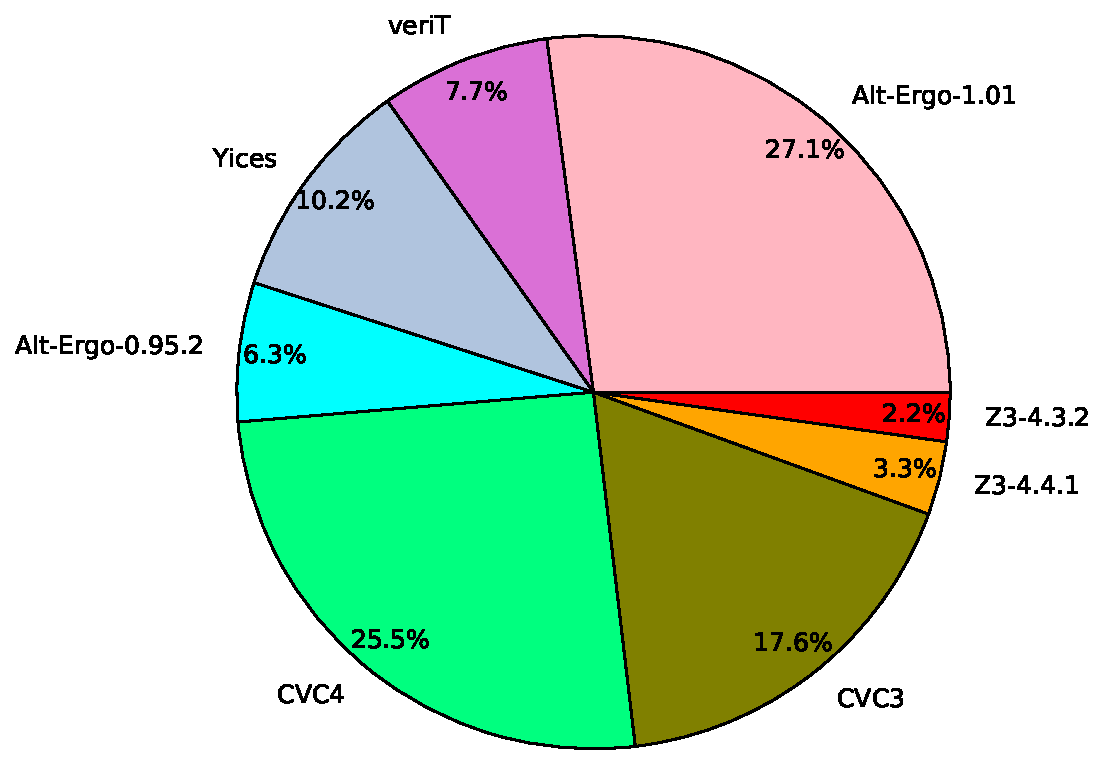
\includegraphics[width=0.8\linewidth]{Figures/pie}
\caption[Relative solver portfolio contributions]{Relative solver portfolio contributions}
\label{fig:pie}
\end{figure}
Figure \ref{fig:pie} shows the normalised contribution statistics for each solver in the portfolio.
Each solver's percentage represents the impact its exclusion has on \textsf{Best Ranking}'s accumulated cost across the entire dataset, relative to the other solvers.
It is unsurprising that Alt-Ergo-1.01 and CVC4 contribute most to the portfolio: these solvers can prove the most uniquely-provable POs (according to Table \ref{table:unique}).  
It is somewhat unexpected that veriT and Yices contribute more than either version of Z3, given that they can prove less goals overall (Table \ref{table:avgtimes}).
This implies that (i) Z3 does not perform significantly better than other solvers for provable goals, (ii) veriT and Yices prove goals in a very short time and (iii) for goals not provable by any of these solvers, veriT and Yices return a better answer in a shorter time.

It is logical that earlier versions of solvers contribute less than more recent versions. 
Alt-Ergo-0.95.2 contributes significantly less than Alt-Ergo-1.01: we deduce that the earlier version takes more time to return a worse answer for \textit{Hard} POs than the update.
Nevertheless, including multiple versions of solvers improves prediction accuracy and ultimately makes \textsf{Where4} a more flexible tool for the user.     


\section{Predictor Selection Results}

\label{sec:pred-results}

In Table \ref{table:predselection} we list the cross-validation results for all six trained prediction models (with discretised and/or weighted variants where applicable).
We compare these  with the three theoretical ranking strategies introduced in Sec. \ref{sec:strategies}.
For each of the five Evaluation Criteria EC1-5, the best-performing algorithm is marked in bold with an asterisk. 

\subsection{EC1: Time}

The first result column, labelled \textbf{Time (secs)}, shows the average time taken for the ranking of solvers returned by the model/strategy to return a \textit{Valid} / \textit{Invalid} response (if such a response was in the set of solver answers -- see Algorithm \ref{algo:rank}).

If there is no \textit{Valid} / \textit{Invalid} response in the set, the time will be the same for any ordering of the solvers (ie. all eight will be called). 
We do not ignore the time taken for the response to be returned.

\subsection{EC2: $R^2$ Score}

The second numeric column of Table \ref{table:predselection} shows
the $R^2$ score (or coefficient of determination), which is an established evaluation criterion. 
It measures how well regression models can predict the variance of dependent / response variables. 
The maximum $R^2$ score is 1 but the minimum can be negative. Note that the theoretical strategies return rankings rather than individual solver costs. 
For this reason, $R^2$ scores are not applicable.

The $R^2$ score is calculated by the following formula
\begin{equation}
\label{r2}
R^2 = 1-\frac{\Sigma(y_i - \hat{y})^2}{\Sigma(y_i - \bar{y})^2}
\end{equation}
which can be interpreted as ``the sum of squared error of the predictions divided by the sum of the squared mean".  
In Formula \ref{r2}, $y_i -\hat{y}$ denotes the distance of the predicted value $\hat{y}$ from the actual value $y$ for data point $i$.
$\bar{y}$ is the mean value from the set of actual values (which in our case is a two-dimensional array of solver scores).
We used the Sci-Kit Learn implementation of this formula, which allows $\bar{y}$ to be set to the weighted average of the outputs for multi-output instances.
We applied uniform weighting to all outputs; meaning the variance of the individual solvers' scores was not considered. 

     



\begin{table}
	\caption[Predictor Selection Results]{ Predictor Selection Results. * indicates the best result among the prediction models }
	
	\begin{adjustbox}{angle=90} 
		\begin{tabularx}{0.9\textheight}{@{}lrrZZZZZ@{}}
			{} & \textbf{Discretised} & \textbf{Weighted} & \textbf{Time (secs)} & $R^2$ & \textbf{nDCG} &  \textbf{MAE} &  \textbf{Reg-error} \\
			\midrule
			\textsf{Best Ranking}  &  &  &     12.59 &    - &  1.00  & 0.00 &        0.00 \\
			\textsf{Random Ranking} & &  &     19.06 &   - &  0.36  & 2.62 &       50.77 \\
			\textsf{Worst Ranking}  & &  &     30.23 &   - &  0.00  & 4.00 &       94.57 \\
			\midrule
			\multirow{4}{*}{Decision Tree}  & \xmark & \xmark     &     16.37 & 0.09 &  0.49 &    2.08 &       45.00 \\
			& \cmark & \xmark     &     15.90 &  -0.18 & 0.43 &  2.27 &       42.65 \\
			& \xmark & \cmark     &     15.81 &  -0.06 & 0.48 &  2.09 &       41.14 \\
			& \cmark & \cmark &     15.75 &  -0.17 & 0.43 &  2.25 &       41.80 \\
			\midrule
			\multirow{2}{*}{k-Nearest Neighbours} & \xmark & \xmark          &     15.40 & 0.17 & \textbf{*0.55} &    \textbf{*1.90} &       40.65 \\
			& \cmark & \xmark          &     15.49 &  -0.19 & 0.44 &  2.26 &       41.47 \\
			\midrule
			\multirow{4}{*}{Linear Regression}  & \xmark & \xmark                        &     15.60 &  -0.11 & 0.41 &  2.45 &       49.70 \\
			& \cmark & \xmark                     &     15.74 &  -0.30 & 0.41 &  2.46 &       49.12 \\
			& \xmark & \cmark                 &     15.78 &  -0.32 & 0.41 &  2.43 &       49.72 \\
			& \cmark & \cmark             &     15.80 &  -0.26 & 0.41 &  2.45 &       50.12 \\
			\midrule
			\multirow{4}{*}{Support Vector Regressor}  & \xmark & \xmark                           &     15.59 &   0.15 & 0.49 &  2.31 &       46.17 \\
			& \cmark & \xmark                        &     15.61 &  -0.23 & 0.43 &  2.31 &       43.17 \\
			& \xmark & \cmark                    &     15.35 &  -0.00 & 0.46 &  2.26 &       41.65 \\
			& \cmark & \cmark                &     15.53 &  -0.19 & 0.44 &  2.26 &       43.17 \\
			\midrule
			\multirow{4}{*}{Random Forest}   & \xmark & \xmark         &     14.99 &  \textbf{*0.28} & 0.48 &   2.09 &       39.63 \\
			& \cmark & \xmark         &     15.04 &  -0.18 & 0.47 &  2.13 &       39.20 \\
			& \xmark & \cmark     &     \textbf{*14.88} &   0.20 & 0.49 &  2.10 &       \textbf{*38.26} \\
			& \cmark & \cmark &     15.03 &  -0.15 &  0.49 & 2.11 &       38.66 \\
			\midrule
			\multirow{4}{*}{Ridge Regression}  & \xmark & \xmark                          &     15.55 &  -0.09 & 0.41 &  2.46 &       49.85 \\
			& \cmark & \xmark                         &     15.65 &  -0.30 & 0.41 &  2.47 &       49.41 \\
			& \xmark & \cmark                     &     15.58 &  -0.08 & 0.40 &  2.49 &       50.12 \\
			& \cmark & \cmark                 &     15.64 &  -0.22 & 0.40 &  2.50 &       50.69 \\
			
		\end{tabularx}
	\end{adjustbox}
	\label{table:predselection}
\end{table}

\subsection{EC3: Normalised Distributed Cumulative Gain}

\label{sub:ndcg}

The third numeric column of Table \ref{table:predselection} shows the 
Normalised Discounted Cumulative Gain (\textbf{nDCG}), which is commonly used to evaluate the accuracy of rankings in the search engine and e-commerce recommender system domains \cite{NDCG}. 
Here, emphasis is placed on correctly predicting items higher in the ranking. For a general ranking of length $p$, it is formulated as:

\begin{equation}
\small
nDCG_p = \frac{DCG_p}{IDCG_p}
\quad\text{ where }\quad
DCG_p = \sum_{i=1}^{p} \frac{2^{rel_i} - 1}{log_2(i+1)}
\label{eq:ndcg}
\end{equation}

where $rel_i$ refers to the relevance of element $i$ with regard to a ground truth ranking, and we take each solver's relevance to be inversely proportional to its rank index.  
In our case, $p = 8$ (the number of SMT solvers).  
The $DCG_p$ is normalised by dividing it by the maximum (or \textit{idealised}) value for ranks of length $p$, denoted $IDCG_p$. 
As our solver rankings are permutations of the ground truth (making $nDCG$ values of zero impossible), the values in Table \ref{table:predselection} are further normalised to the range [0..1] using the lower $nDCG$ bound for ranks of length eight -- found empirically to be 0.4394.

We illustrate our use of this criterion with a small example. 
Take a ground truth ranking of eight items sorted in decreasing relevance as
\[ A > B > C > D > E > F > G > H. \]
We take each item's \textit{relevance} to be inversely-proportional to its rank position:
\[rel_A=8, rel_B=7, rel_C=6, rel_D=5, rel_E=4, rel_F=3, rel_G=2, rel_H=1.\]
The predicted ranking of these items is
\[ B > A > C > F > D > E > G > H .\]
Applying Equation \ref{eq:ndcg} to these values gives us an $nDCG$ value of
\[
\frac{127}{1.0} + \frac{255}{1.58} + \frac{63}{2.0} + \frac{7}{2.32} + \frac{31}{2.58} + \frac{15}{2.81} + \frac{3}{3.0} + \frac{1}{3.17} = 341.053. 
\]
It can be shown that $IDCG_8 = 389.591$ which makes the un-normalised $nDCG$ value for the predicted ranking 0.875. Using the lower bound of 0.4394 to normalise this value to the range $\left[0, 1 \right]$ (accounting for permutations of length 8) gives us a final $nDCG$ score of 0.778. 

The nDCG metric is best understood in relation to other rankings in the same problem domain: a score of say, 0.5, is meaningless in isolation.
For this reason, we provide Table \ref{table:ndcg} so that the reader may gain an intuitive understanding of this metric as we use it.

\begin{table}
	\centering
	\caption[Illustration of various nDCG scores]{Illustration of various nDCG scores (normalised for permutations of length eight)}
	
	
	\begin{tabularx}{0.7\textwidth}{@{}lZ@{}}
		\toprule
		\textsc{Permutation} & \textsc{nDCG score} \\
		\midrule
		\textbf{ABCDEFGH} & \textbf{1.0} \\
		\textbf{ABCDEF}\textit{HG} & 0.9998\\
		\textbf{ABCD}\textit{FE}\textbf{GH} & 0.9989\\
		\textbf{AB}\textit{DC}\textbf{EFGH} & 0.9899\\
		\textit{BA}\textbf{CDEFGH} & 0.7848\\
		\textbf{ABCD}\textit{HGFE} & 0.9950\\
		\textit{DCBA}\textbf{EFGH} & 0.3809\\
		\textit{HGFEDCBA} & 0.0\\
		\bottomrule
	\end{tabularx}
	\label{table:ndcg}
\end{table}

\subsection{EC4: Mean Average Error}

Table \ref{table:predselection}'s fourth numeric column shows the 
$MAE$ (Mean Average Error) -- a ranking criterion which can also be used to measure string similarity. It measures the average distance from each predicted rank position to the solver's index in the ground truth.

Using the same predicted and actual rankings as the $nDCG$ example, we calculate the $MAE$ to be:
\[
	MAE = \frac{1 + 1 + 0 + 2 + 1 + 1 + 0 + 0}{8} = 0.75
\]

The Mean Average Error is a good measure of overall ranking accuracy, but it fails to take into account that in many use cases -- including \textsf{Where4} -- it is often the highest-ranking items that are the most important to predict accurately. 

\subsection{EC5: Regression Error}

The rightmost column of Table \ref{table:predselection} (labelled \textbf{Reg. error}) lists the average regression error per instance. 
We illustrate the calculation of the regression error with a small example. For two testing instances, the predicted and actual costs for three solvers are: 
\[ \left( \begin{array}{ccc}
0.5 & 10.0 & 5.0 \\
0.4 & 5.5 & 10.0  \end{array} \right) = \text{predicted};
\left( \begin{array}{ccc}
0.6 & 9.0 & 8.0 \\
0.7 & 9.5 & 7.0 \end{array} \right) = \text{actual}\]
which gives a per-instance regression error of
\[ \left( \begin{array}{c}
0.1 + 1.0 + 3.0 \\
0.3 + 4.0 + 3.0
\end{array}  \right) = 
\left( \begin{array}{c}
4.1 \\
7.3
\end{array}  \right) \] 
taking the average of the two instances' regression error, 4.1 and 7.3, gives 5.7.
It is this average error between predicted cost and actual cost for eight solvers which is listed in the rightmost column.

The regression error should be treated with a note of caution, however, as the relative ranking of solvers -- which we argue is the most important prediction -- is not explicitly taken into account.
This qualification also applies to the MAE and $R^2$ score criteria. 
Note that when the predictions and actual costs are sorted in increasing order the best-performing solver is predicted correctly for both instances in the previous example.
The entire ranking of solvers is predicted correctly in the first instance.

\subsection{Properties of multi-output problems}
\label{sub:multi}

An interesting feature of all the best-performing models in Table \ref{table:predselection} -- Random Forests, K-Nearest Neighbours, Decision Trees -- is their ability to predict \textit{multi-output} variables. 
In contrast to Support Vector Machines, for example, which must predict the cost for each solver individually, an algorithm which supports multi-output problems can predict each solver's cost simultaneously. 
Not only is this method more efficient (by reducing the number of estimators required), but it has the ability to account for the correlation of the response variables. 
This is a useful property in the software verification domain where certain goals are not provable and others are trivial for SMT solvers. 
Multiple versions of the same solver can also be expected to have highly correlated scores.

A more general survey of multi-output regression and how various ML algorithms can either be adapted or extended for this use case is provided by Borchani et al. \cite{multisurvey}.

\subsection{The chosen model}
\label{sec:chosen}


\begin{table}
	\caption[Relative importance of features for \where]{Relative importance of each feature in the \textsf{Where4}Random Forest model}
	
	
	\begin{tabularx}{\textwidth}{@{}lr|c|lr@{}}
		\toprule
		\textsc{Feature} & \textsc{Importance (\%)} & & 
		\textsc{Feature} & \textsc{Importance (\%)}  \\
		\midrule
		\texttt{func} & 19.63 & & \texttt{divisor} & 2.66 \\
		\texttt{avg-op-arity} &  11.05 & & \texttt{n-ops} & 2.48 \\
		\texttt{int} & 8.96 & & \texttt{not} & 1.15 \\
		\texttt{forall} & 7.19 & & \texttt{if} & 1.07 \\
		\texttt{and} & 6.02 & & \texttt{case} & 0.99 \\
		\texttt{depth} & 5.70 & & \texttt{wild} & 0.84 \\
		\texttt{var} & 4.84 & & \texttt{false} & 0.37 \\
		\texttt{impl} & 4.72 & & \texttt{or} & 0.36 \\
		\texttt{size} & 4.31 & & \texttt{iff} & 0.33 \\
		\texttt{let} & 4.03 & & \texttt{eps} & 0.13 \\
		\texttt{n-quants} & 3.70 & & \texttt{true} & 0.12 \\
		\texttt{n-preds} & 3.27 & & \texttt{exists} & 0.07 \\
		\texttt{zero-ar} & 3.03 & & \texttt{float} & 0.00 \\
		\texttt{n-branches} & 2.97 & & \texttt{as} & 0.00 \\
		\bottomrule	
	\end{tabularx}
	\label{table:importances}
\end{table}


After inspecting the results for all trained models (summarised in Table \ref{table:predselection}), we can see that Random Forests \cite{RandomForests} perform well, relative to other methods. 
They score highest for three of the five criteria (shown in bold with an asterisk) and have generally good scores in the others.
Based on these results, we selected Random Forests as the choice of algorithm to use in \where.
We chose to implement a Random Forest model which does not use discretisation or instance weighting. 
Inspecting the results from the entire range of algorithms shows that, in general, the best-performing models do not use these techniques.

The k-Nearest Neighbours model, while coming top for two important criteria, scored poorly in the \textbf{Time} category.
This result leads us to conclude that k-Nearest Neighbours can often predict good rankings but the instances on which it performs badly are very expensive in terms of time.
Overall, the Random Forest model is the most consistent and reliable predictor.

Before discussing the implementation of \textsf{Where4}in the next chapter, we shall investigate the properties of the Random Forest model after it was fit on the entire training dataset.

Table \ref{table:importances} shows the relative importance of each predictor variable for decision-making in the Random Forest model. 
Every time a split of a node is made on a feature the impurity criterion for the two descendent nodes is less than the parent node. 
This criterion is called the \textit{Gini impurity} \cite{RandomForests}. 
The percentages correspond to the proportion of the \textit{Gini} decrease accounted for splitting by each feature.
This data is part of Sci-Kit Learn's implementation of Decision Trees and Random Forests. 

It can be seen that the number of functions in each PO is by far the most important factor in determining each solver's cost, with the average branching factor of functions and other operators also being important.
It is somewhat surprising that the number of integer constants is one of the more important factors while the number of floating point constants is relatively unimportant.
This may be due to the fact that there are more integer-based POs in our dataset than those which use floating point numbers.
This reasoning may also account for the fact the universal quantifiers (\texttt{forall}) rank higher than existential (\texttt{exists}) quantifiers.



\section{Summary}

This chapter began by motivating the use of portfolio-solving in the \textsf{Why3} system by showing that more files, theories and goals can be proven by using the best-performing solver on a per-goal basis.
We then gave a tour of the prediction approaches considered for use in \where.
We decided to use a regression method to predict each solver's \textit{cost} -- a value designed to account for solver response as well as the time taken to return the response. 

A number of ranking strategies and evaluation criteria were described in Sec. \ref{sec:strategies} and Sec. \ref{sec:pred-results} respectively.
%We will encounter these concepts again during the evaluation of \textsf{Where4}on test data in Chapter \ref{Evaluation}.
In this chapter, we used them to compare various trained models and found Random Forests to be the best choice for implementation in \where.

Some properties of the trained Random Forest model were then discussed.
The choice of prediction model has an obvious importance on \where's  implementation and success as a predictor. 
We give more details of this implementation in the next chapter.  



